%
% c.tex -- slide template
%
% (c) 2021 Prof Dr Andreas Müller, OST Ostschweizer Fachhochschule
%
\bgroup
\begin{frame}[t]
\setlength{\abovedisplayskip}{5pt}
\setlength{\belowdisplayskip}{5pt}
\frametitle{Drehgruppen}
\vspace{-25pt}
\begin{columns}[t,onlytextwidth]
\begin{column}{0.33\textwidth}
\begin{block}{$C_n$}
\begin{center}
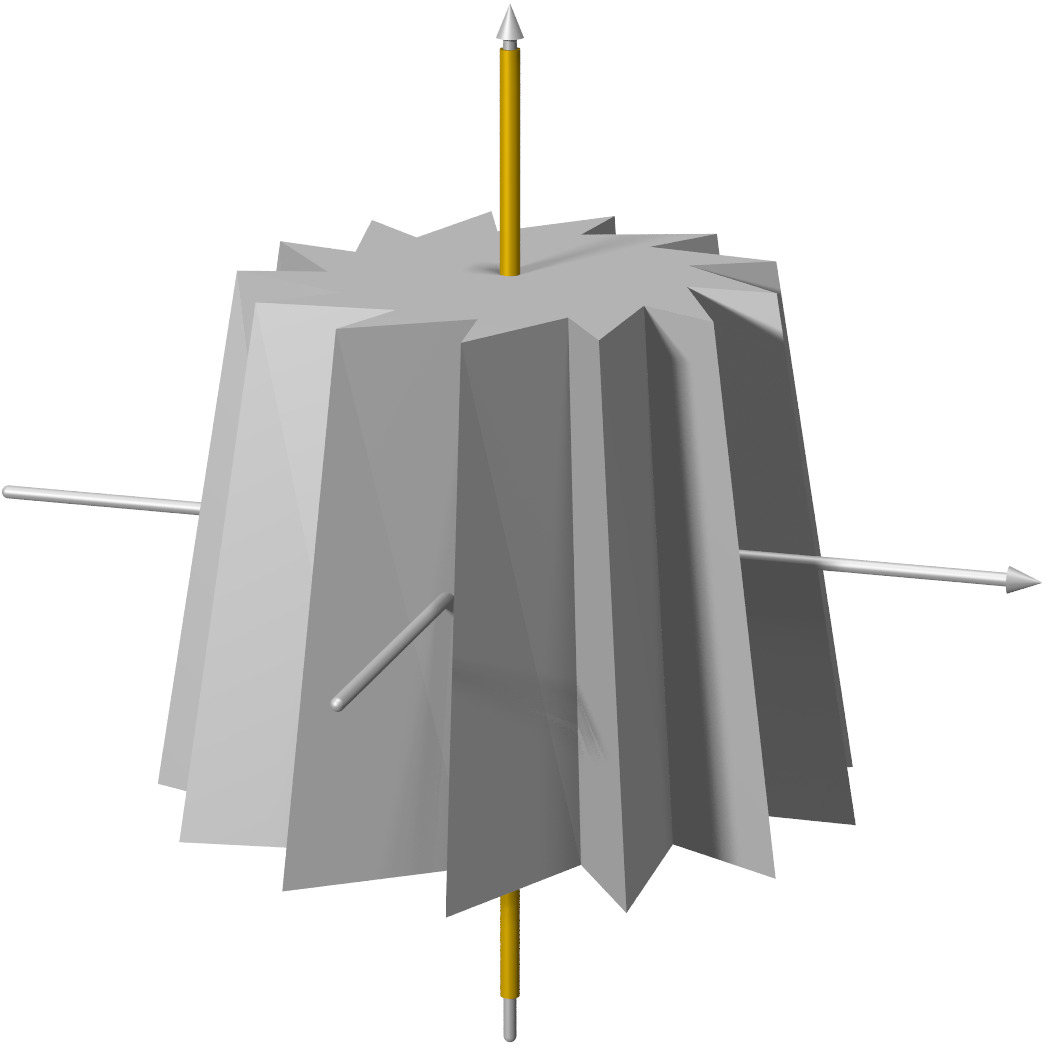
\includegraphics[width=\textwidth]{../slides/6/punktgruppen/images/cn.jpg}
\end{center}
\begin{itemize}
\item Eine $n$-zählige Achse
\end{itemize}
\end{block}
\end{column}
\begin{column}{0.33\textwidth}
\uncover<2->{%
\begin{block}{$C_{nv}$}
\begin{center}
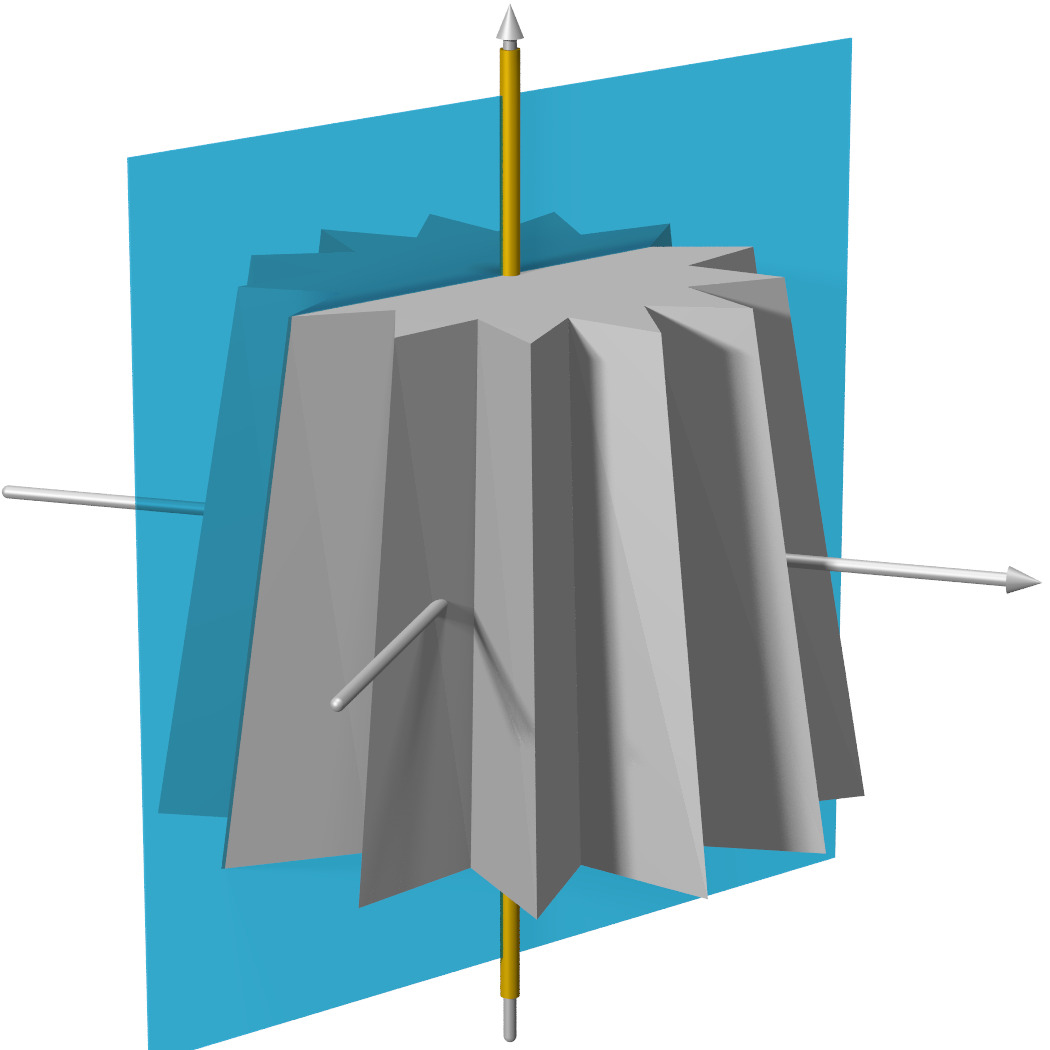
\includegraphics[width=\textwidth]{../slides/6/punktgruppen/images/cnv.jpg}
\end{center}
\begin{itemize}
\item Eine $n$-zählige Achse
\item $n$ dazu senkrechte Symmetrieebenen
\end{itemize}
\end{block}}
\end{column}
\begin{column}{0.33\textwidth}
\uncover<3->{%
\begin{block}{$C_{nh}$}
\begin{center}
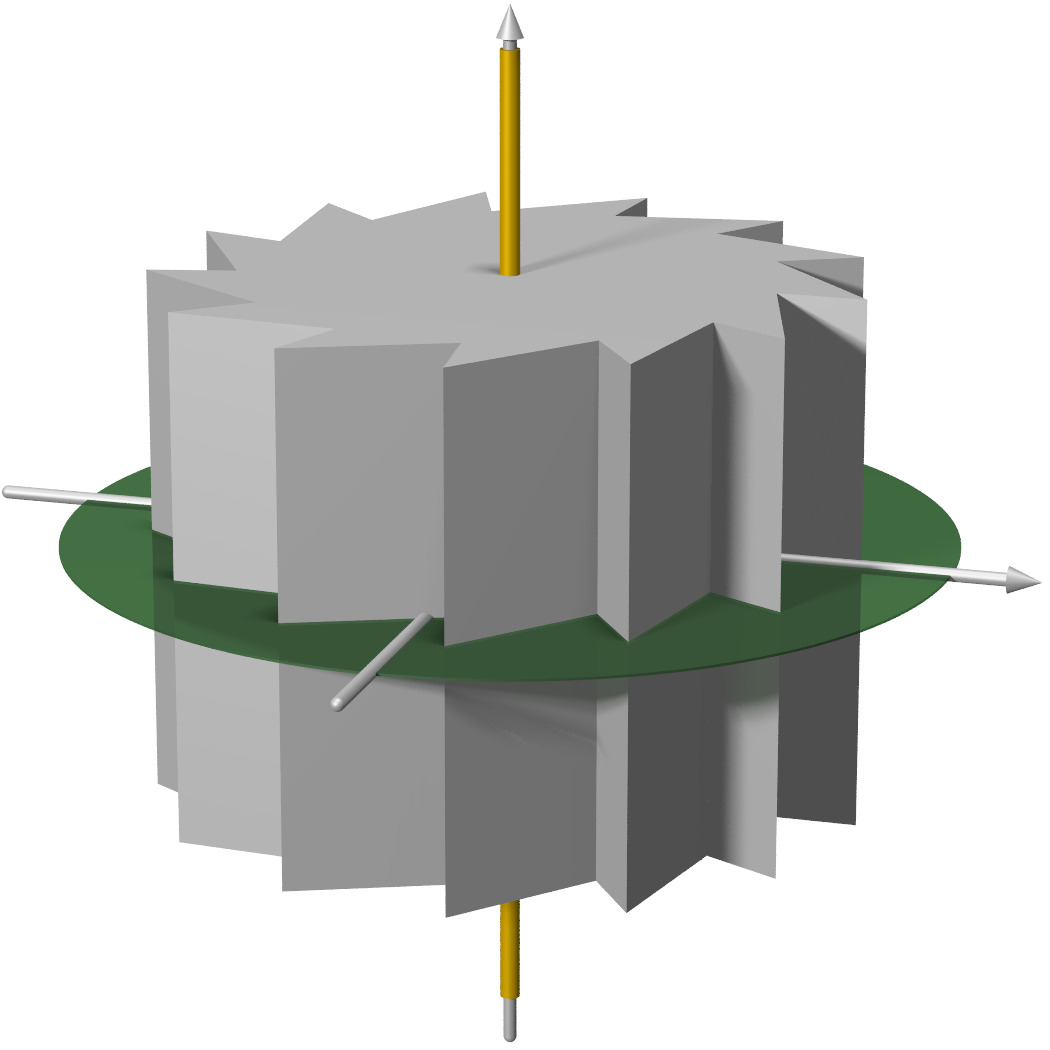
\includegraphics[width=\textwidth]{../slides/6/punktgruppen/images/cnh.jpg}
\end{center}
\begin{itemize}
\item Eine $n$-zählige Achse
\item Eine dazu senkrechte Spiegelebene
\end{itemize}
\end{block}}
\end{column}
\end{columns}
\end{frame}
\egroup
